\subsubsection{UC-1 Registrazione}
		\begin{figure}[h]
			\centering
			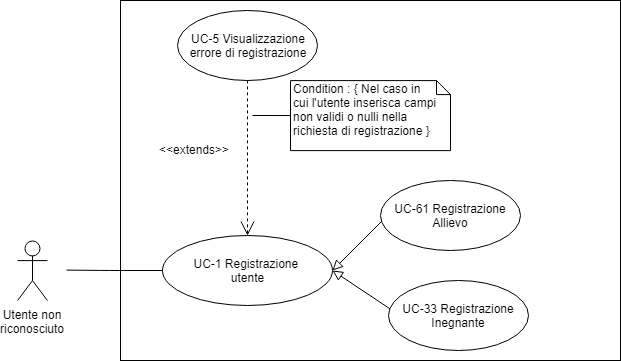
\includegraphics[scale=0.7]{images/UC-1.png}
			\caption{UC-1 Registrazione}
		\end{figure}			
\begin{itemize}
		\item \textbf{Attori: }Utente non registrato
		\item \textbf{Precondizione: }L'utente si trova nella vista di registrazione dell'applicazione.
		\item \textbf{Postcondizione: }L'utente è registrato o come allievo o come insegnante.
		\item \textbf{Scenario principale: }
		\begin{enumerate}
		\item l'utente ha scelto di registrarsi al sistema, quindi di creare un nuovo profilo. 
		\item l'utente dovrà scegliere la tipologia di utente, insegnante/allievo. 
		\item l'utente inserirà nome, cognome, username, email e password;
		\item l'utente fornirà il nome della scuola a cui appartiene e la città; 
		\item l'utente conferma la registrazione.
		\end{enumerate}
		\item \textbf{Estensioni: }
		\begin{itemize}
			\item 5.a Nel caso in cui l'utente tenti l'inserimento di campi non validi vedrà comparire dei messaggi d'errore (UC-5).
			\item 5.b un utente che si è registrato come insegnante deve attendere la conferma dela registrazione dell'amministratore (UC-4).
		\end{itemize}
	\end{itemize}
\subsubsection{UC-2 Autenticazione}
		\begin{itemize}
			\item Attori: Utente non autenticato;
			\item Precondizione: l'utente si trova nella vista di autenticazione dell'applicazione;
			\item Postcondizione: l'utente ha eseguito l'accesso con il proprio ruolo.
			\item Scenario principale:
				\begin{enumerate}
					\item l'utente inserisce la propria email e password;
					\item l'utente conferma l'accesso.
				\end{enumerate}
				\item Estensioni:
				\begin{itemize}
					\item 2.a Nel caso in cui l'utente tenti l'inserimento di campi non validi vedrà comparire messaggi d'errore (UC-5).
				\end{itemize}
		\end{itemize}
		
	\subsubsection{UC-3 Modifica profilo}
		\begin{figure}[h]
			\centering
			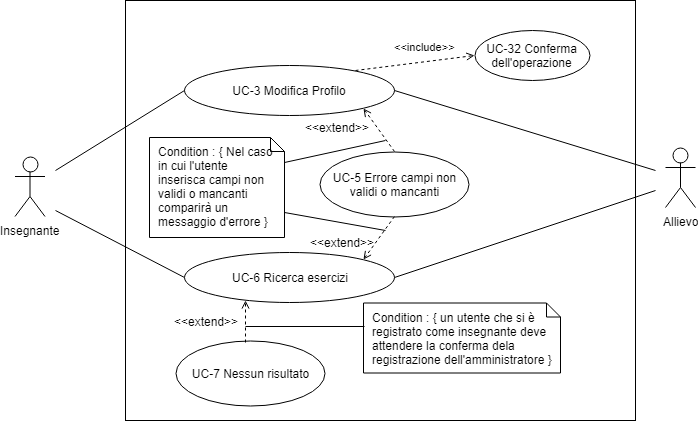
\includegraphics[scale=0.7]{images/UC-3.png}
			\caption{UC-3 Modifica profilo e UC-6 Ricerca esercizi}
		\end{figure}
		\begin{itemize}
			\item Attori: insegnante, allievo;
			\item Precondizione: l'utente si trova nella vista di modifica dei dati del proprio profilo;
			\item Postcondizione: l'utente ha modificato i propri dati personali.
			\item Scenario principale:
				\begin{enumerate}
					\item l'utente modifica username, password, scuola, città;
					\item l'utente conferma la moodifica.
				\end{enumerate}
				\item Estensioni:
				\begin{itemize}
					\item 2.a nel caso in cui l'utente tenti l'inserimento di campi non validi vedrà comparire messaggi d'errore (UC-5).
				\end{itemize}
		\end{itemize}
\subsubsection{UC-4 Verifica richiesta insegnante}
		\begin{itemize}
			\item Attori: amministratore;
			\item Precondizione: l'amministratore si trova nella vista di amministrazione dell'applicazione;
			\item Postcondizione: l'amministratore ha confermato l'utente richiedente il ruolo di insegnante.
			\item Scenario principale:
				\begin{enumerate}
					\item l'amministratore visualizza la lista degli utenti che richiedono il ruolo di insegnante;
					\item l'amministratore acceta o rifiuta l'utente selezionato.
				\end{enumerate}
		\end{itemize}

\subsubsection{UC-5 Errore campi non validi o mancanti}
\begin{itemize}
\item \textbf{Attori: } utente 
\item \textbf{Precondizione: }L'utente ha inserito dei campi non validi.
\item \textbf{Postcondizione: }Il sistema mostra un messaggio d'errore per spronare l'utente a ricontrollare i campi non validi.
\item \textbf{Scenario principale: }
		\begin{enumerate}
		\item L'utente ha provato a inserire dei campi non validi.
		\item All'utente viene mostrato un messaggio d'errore che invita a ricontrollare i campi non validi.
		\end{enumerate}
\end{itemize}
\subsubsection{UC-6 Ricerca esercizi}
		\begin{itemize}
			\item Attori: allievo, insegnante;
			\item Precondizione: l'utente si trova nella vista principale dell'applicazione;
			\item Postcondizione: l'utente ottiene una lista degli esercizi filtrati.
			\item Scenario principale:
				\begin{enumerate}
					\item l'utente accede all'area dedicata alla ricerca degli esercizi;
					\item l'utente scrive la frase nella barra di ricerca;
					\item l'utente seleziona i filtri UC-6.1.
					\item l'utente avvia la ricerca.
				\end{enumerate}
			\item Estensioni:
				\begin{itemize}
					\item 2.a Nel caso in cui l'utente tenti l'inserimento di campi non validi vedrà comparire messaggi d'errore (UC-5).
					\item 3.a Se non c'è nessun risultato viene visualizzato un messaggio: ``nessun risultato trovato" (UC-7).
				\end{itemize}
		\end{itemize}
\subsubsection{UC-6.1 Filtraggio esercizi }
\begin{itemize}
\item Attori: allievo, insegnante;
			\item Precondizione: l'utente si trova nella vista di ricerca degli esercizi dell'applicazione;
			\item Postcondizione: l'utente ha selezionato i filtri per la ricerca.
			\item Scenario principale:
				\begin{enumerate}
					\item l'utente può selezionare l'autore degli esercizi desiderati;
					\item l'utente può selezionare il livello di difficoltà degli esercizi;
					\item l'utente può selezionare gli argomenti degli esercizi
				\end{enumerate}

\end{itemize}
\subsubsection{UC-7 Visualizzazione messaggio ``nessun risultato trovato"}
\begin{itemize}
		\item \textbf{Attori: } Insegnante, Allievo, Sviluppatore
		
		\item \textbf{Precondizione: }L'utente ha avviato la ricerca. 
		\item \textbf{Postcondizione: }L'utente visualizza un messaggio: ``nessun risultato trovato".
		\item \textbf{Scenario principale: }
		\begin{enumerate}
			\item Viene mostrato un messaggio: ``nessun risultato trovato".
		\end{enumerate}
\end{itemize}

\subsubsection{UC-8 Eliminazione di un utente}
	\begin{itemize}
			\item Attori: amministratore;
			\item Precondizione: l'amministratore si trova nella vista di amministrazione dell'applicazione;
			\item Postcondizione: l'amministratore ha eliminato l'utente desiderato.
			\item Scenario principale:
				\begin{enumerate}
					\item l'amministratore indica l'utente da eliminare;
					\item l'amministratore conferma l'eliminazione dell'utente selezionato.
				\end{enumerate}
		\end{itemize}
	
\subsubsection{UC-9 Modifica soluzione}
\begin{figure}[h]
			\centering
			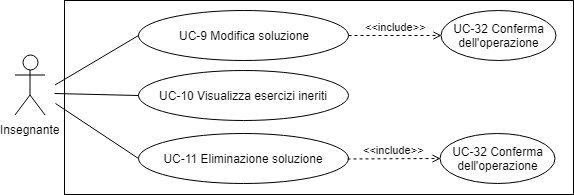
\includegraphics[scale=0.7]{images/UC-9.png}
			\caption{UC-9 Modifica soluzione, UC-10 Visualizzazione esercizi inseriti, UC-11 Eliminare una soluzione di un esercizio}
		\end{figure}
\begin{itemize}

\item \textbf{Attori: }Insegnante
\item \textbf{Precondizione: }L'insegnante ha selezionato un esercizio di cui ha fornito una soluzione.
\item \textbf{Postcondizione: }La soluzione inserita è stata modificata.
\item \textbf{Scenario principale: }
		\begin{enumerate}
		\item L'insegnante visualizza i campi con la vecchia soluzione.
		\item L'insegnante modifica i campi che ritiene errati.
		\item L'insegnante conferma la modifica.
		\end{enumerate}
\end{itemize}

\subsubsection{UC-10 Visualizzazione esercizi inseriti}
\begin{itemize}
\item \textbf{Attori: }Insegnante
		\item \textbf{Precondizione: }L'insegnante si trova nell'area del suo profilo.
		\item \textbf{Postcondizione: }L'insegnante visualizza una lista di esercizi inseriti. 
		\item \textbf{Scenario principale: }
		\begin{enumerate}
		\item L'insegnante accede alla vista degli esercizi inseriti.
		\end{enumerate}
	\end{itemize}
	
\subsubsection{UC-11 Eliminare una soluzione di un esercizio}
\begin{itemize}
\item \textbf{Attori: }Insegnante
		\item \textbf{Precondizione: }L'insegnate ha selezionato la soluzione da eliminare.
		\item \textbf{Postcondizione: }La soluzione selezionata viene eliminata. 
		\item \textbf{Scenario principale: }
		\begin{enumerate}
		\item L'utente sceglie una soluziona da eliminare.
		\item La soluzione scelta viene eliminata.
		\end{enumerate}
	\end{itemize}

\subsubsection{UC-12 Inserimento esercizio}
\begin{figure}[h]
			\centering
			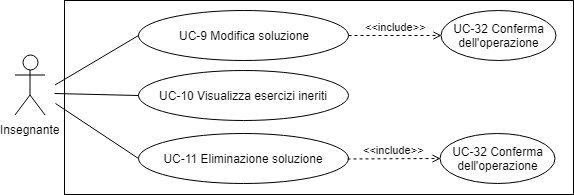
\includegraphics[scale=0.7]{images/UC-9.png}
			\caption{UC-12 Inserimento esercizio}
		\end{figure}
	\begin{itemize}
		\item \textbf{Attori: }Insegnante
		\item \textbf{Precondizione: }L'insegnante è nella vista di inserimento di un nuovo esercizio.
		\item \textbf{Postcondizione: }L'esercizio è stato inserito.
		\item \textbf{Scenario principale: }
		\begin{enumerate} 
		\item L'insegnante inserisce la frase;
		\item L'insegnante inserisce la soluzione UC-12.1;
		\item L'insegnante inserisce la difficoltà;
		\item L'insegnante inserisce gli argomenti UC-12.2;
		\item L'insegnante conferma l'inserimento.
		\end{enumerate}
		\item \textbf{Estensioni: }
		\begin{itemize}
		\item 6.a Nel caso in cui i campi compilati presentino errori verrà mostrato un messaggio d'errore (UC-5).
		\end{itemize}
	\end{itemize}

\subsubsection{UC-12.1 Inserimento di una soluzione}
\begin{itemize}
\item \textbf{Attori: }Insegnante
\item \textbf{Precondizione: }L'insegnante è nella vista di inserimento di un nuovo esercizio.
\item \textbf{Postcondizione: }L'insegnante ha inserito la propria soluzione.
\item \textbf{Scenario principale: }
		\begin{enumerate} 
		\item L'insegnante visualizza i campi proposti dal generatore automatico. 
		\item L'insegnante può modificare i campi che ritiene errati.
		\item L'insegnante seleziona lo stato della soluzione inserita, pubblica o privata;
		\item L'insegnante conferma la soluzione.
		\end{enumerate}	
\end{itemize}

\subsubsection{UC-12.2 Inserimento argomenti}
\begin{itemize}
\item \textbf{Attori: }Insegnante

\item \textbf{Precondizione: }L'insegnante sta inserendo un esercizio, gli viene richiesta la compilazione di una lista di argomenti presenti nell'esercizio.
\item \textbf{Postcondizione: }L'insegnante ha selazionato gli argomenti trattati nell'esercizio.
\item \textbf{Scenario principale: }
		\begin{enumerate}
		\item L'insegnante sta inserendo un esercizio. 
		\item L'insegnante seleziona gli argomenti che vengono toccati nell'esercizio. 
		\end{enumerate}
\end{itemize}

\newpage


					
					
					
\subsection{Attore Allievo}
	\subsubsection{UC-13 Svolgimento esercizio}
	\begin{figure}[h]
			\centering
			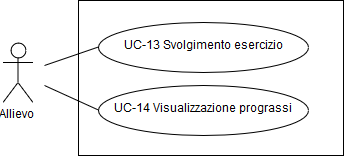
\includegraphics[scale=0.7]{images/UC-13.png}
			\caption{UC-13 Svolgimento esercizio, UC-14 Visualizzazione progressi}
	\end{figure}	
	\begin{itemize}
	\item Attori: Allievo
			\item Precondizione:  L'allievo visualizza la lista degli esercizi ricercati.
			\item Postcondizione: L'allievo visualizza la valutazione dell'esercizio.
			\item Scenario principale:
			\begin{enumerate}
				\item l'allievo seleziona l'esercizio da svolgere (UC-13.1).
				\item l'allievo compila i campi (UC-13.2).
				\item l'allievo conferma i dati inseriti.
				\item l'allievo visualizza la valutazione (UC-13.3).
			\end{enumerate}
	\end{itemize}
			
	\subsubsection{UC-13.1 Selezione esercizio}
	\begin{figure}[h]
			\centering
			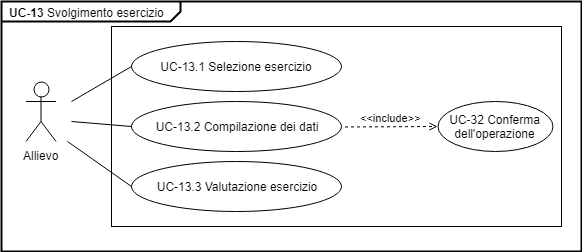
\includegraphics[scale=0.7]{images/UC-13_1.png}
			\caption{UC-13.1 Selezione esercizio, UC-13.2 Compilazione dei dati, UC-13.3 Valutazione esercizio}
	\end{figure}
	\begin{itemize}
			\item Attori: Allievo
			\item Precondizione: L'allievo visualizza la lista degli esercizi ricercati.
			\item Postcondizione: L'allievo visualizza la vista per l'esecuzione dell'esercizio.
			\item Scenario principale:
				\begin{enumerate}
					\item l'allievo indica (scrivendola o selezionandola) la frase da svolgere.
					\item l'allievo seleziona il correttore dell'esercizio(insegnante o algoritmo automatico).
					\item l'allievo conferma la selezione.
				\end{enumerate}
			\end{itemize}

	\subsubsection{UC-13.2 Compilazione dei campi}
		\begin{itemize}
			\item Attori: Allievo
			\item Precondizione: l'allievo ha selezionato un esercizio da eseguire;
			\item Postcondizione: l'allievo ha compilato i campi proposti dall'esercizio.
			\item Scenario principale:
				\begin{enumerate}
					\item l'allievo sceglie la classe grammaticale per ogni parola presentata.
					\item l'allievo conferma la soluzione dell'esercizio.
				\end{enumerate}
			\item Estensioni: 
				\begin{itemize}
					\item UC-5 Nel caso in cui l'utente tenti l'inserimento di campi non validi vedrà comparire messaggi d'errore.
				\end{itemize}
		\end{itemize}

	\subsubsection{UC-13.3 Valutazione esercizio}
	\begin{itemize}
			\item Attori: Allievo
			\item Precondizione: L'allievo ha completato l'esecuzione dell'esercizio;
			\item Postcondizione: L'allievo visualizza la valutazione dell'esercizio.
			\item Scenario principale:
				\begin{enumerate}
					\item l'allievo al termine dell'esecuzione dell'esercizio riceve la valutazione.
				\end{enumerate}
			\end{itemize}
			
	\subsubsection{UC-14 Visualizzazione progressi}
	\begin{itemize}
			\item Attori: Allievo
			\item Precondizione: L'allievo si trova nella vista del proprio profilo;
			\item Postcondizione: L'allievo visualizza i progressi svolti fino a quel momento.
			\item Scenario principale:
				\begin{enumerate}
					\item l'allievo visualizza la media delle valutazioni ricevute.
					\item l'allievo visualizza i grafici riguardanti i propri progressi.
					\item l'allievo visualizza il numero di esercizi svolti.
				\end{enumerate}
	\end{itemize}
			

